\iffalse
\let\negmedspace\undefined
\let\negthickspace\undefined
\documentclass[a4,12pt,onecolumn]{IEEEtran}
\usepackage{amsmath,amssymb,amsfonts,amsthm}
\usepackage{algorithmic}
\usepackage{graphicx}
\usepackage{textcomp}
\usepackage{xcolor}
\usepackage{txfonts}
\usepackage{listings}
\usepackage{enumitem}
\usepackage{mathtools}
\usepackage{gensymb}
\usepackage[breaklinks=true]{hyperref}
\usepackage{tkz-euclide}
\usepackage{listings}
\usepackage{circuitikz}
\usepackage{gvv}
\begin{document}
\title{
\Huge\textbf{ GATE 2021 Assignment}\\
\Huge\textbf{EE1205} Signals and Systems\\
}
\large\author{Kurre Vinay\\EE23BTECH11036}
\maketitle
\textbf{Question:}
The exponential Fourier series representation of a continous-time periodic signal x\brak{t} is defined as\\
\begin{center}
$x\brak{t}=\sum\limits_{k=-\infty}^{\infty}a_ke^{jk\omega_0t}$\\
\end{center}
where $\omega_0$ is the fundamental angular frequency of x\brak{t} and the coefficients of the series are $a_k$.The following information is given about x\brak{t} and $a_k$\\
I. x\brak{t} is real and even,having a fundamental period of 6\\
II. The average value of x\brak{t} is 2.\\
III.\begin{align}
 a_k= \begin{cases} 
      k, & 1 \leq k \leq 3 \\
      0, &  k > 3 
   \end{cases}\\
   \end{align}
The average power of the signal x\brak{t} (rounded off to one decimal place) is \underline{\hspace{1cm}}. \\
\hfill(GATE EC 2021)\\
\solution\\
\fi
\begin{table}[ht!]
\begin{center}
\begin{tabular}{|c|c|c|}
   \hline
   variable&value&description\\
   \hline
   $T_0$&6&Fundamental time period\\
   \hline
  $P_{avg}$&-&average power of the signal\\
   \hline
   x\brak{t}&$\sum\limits_{k=-\infty}^{\infty}a_ke^{jk\omega_0t}$&Input signal\\
   \hline
   $a_k$& $\begin{cases} 
      k, & 1 \leq k \leq 3 \\
      0, &  k > 3 
   \end{cases}$&coefficients of the series \\
   \hline
  $a_0$&2&average of x\brak{t}\\
   \hline
\end{tabular}
\caption{Table: Input Parameters}
\end{center}
\end{table}\\
x\brak{t} is even and real so, $a_k$=$a_{-k}$\\
Parswal's Power Theorem\\
Proof
\begin{align}
P&=\frac{1}{T}\int\limits_{\frac{-T}{2}}^{\frac{T}{2}}\left| x\brak{t}^2 \right|dt ,\quad{\left| x\brak{t}^2 \right|=x\brak{t}x^*\brak{t}}\\
P&=\frac{1}{T}\int\limits_{\frac{-T}{2}}^{\frac{T}{2}}x\brak{t}x^*\brak{t}dt \\
x\brak{t}&=\sum\limits_{n=-\infty}^{\infty}C_ne^{jn\omega_0t}\\
P&=\frac{1}{T}\int\limits_{\frac{-T}{2}}^{\frac{T}{2}}\brak{\sum\limits_{k=-\infty}^{\infty}C_ne^{jn\omega_0t}}x^*\brak{t}dt\\
P&=\sum\limits_{n=-\infty}^{\infty}C_n\brak{\frac{1}{T}\int\limits_{\frac{-T}{2}}^{\frac{T}{2}}x^*\brak{t}e^{jn\omega_0t}dt}\\
&=\sum\limits_{n=-\infty}^{\infty}C_nC^*_n\\
\implies P&=\sum\limits_{n=-\infty}^{\infty}\left| C_n \right|^2
\end{align}
By using Parsval's Power Theorem
\begin{align}
\frac{1}{T}\int\limits_{0}^{T}\left| x\brak{t}^2 \right|dt&=\sum\limits_{k=-\infty}^{\infty}\left| a_k \right|^2\\
P_{avg}&=\sum\limits_{k=-\infty}^{\infty}\left| a_k \right|^2\\
&=2\sum\limits_{k=1}^{\infty}\left| a_k \right|^2 +|a_0|^2\\
&=2\sum\limits_{k=1}^{3}\left| a_k \right|^2  +|a_0|^2 \\
&=2\brak{1^2+2^2+3^2}+2^2\\
&=32\\
x\brak{n}&=2\text{Re}\brak{e^{\frac{j\pi t}{3}}+2e^{\frac{2j\pi t}{3}}+3e^{j\pi t}} + 2\\
\implies x\brak{n}&=2\brak{cos\brak{\frac{\pi t}{3}}+2cos\brak{\frac{2\pi t}{3}}+3cos\brak{\pi t}} + 2
\end{align}
The average power of the signal x\brak{t} (rounded off to one decimal place) is $32$
\begin{figure}[ht!]
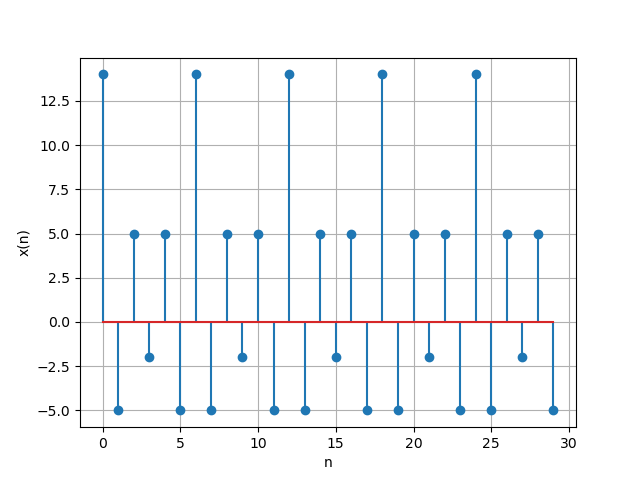
\includegraphics[width=\columnwidth]{2021/EC/39/figs/fig.png}
\caption{\large{STEM PLOT OF $y\brak{n}$}}
\end{figure}

